\chapter{序論}\label{ux5e8fux8ad6}

筆者は卒業制作として、音響遅延線メモリーというコンピューターの初期に使われていた記憶装置を題材にした音響装置作品の制作を行った。\\
音響遅延線という装置の概要については本論で述べることにするが、一連の制作においてはすでに淘汰され使われなくなったメディア装置、その中でも特に記憶装置を取り上げ、現代の技術を取り込み別のメディア装置として再生させるという作品制作のプロセスを取った。

\section{動機と問題意識}\label{ux52d5ux6a5fux3068ux554fux984cux610fux8b58}

今日、デジタルネイティブという言葉が存在するように我々が何か技術を使うときにアナログ、デジタルと言う境目を意識することは少なくなったように思える。また、それに伴い「保存する」ことと「通信する」事の境界は曖昧になりつつ有る。

例えば、MicrosoftのWordに代表される文書作成ソフトをWebブラウザ上で動作させるようにしたGoogle
Docs\footnote{Googleの提供する、ウェブブラウザ上で動作する文書作成ソフト。Wordなどの既存のフォーマットを扱うこともできる。元々2005年にUpstartle社のWritelyというWebサービスから始まり2006年にGoogleが買収しGoogle
  Documentとなった。共同編集機能はサービス開始当初からの特徴であった。\url{https://www.google.co.jp/intl/ja/docs/about/}}では書き込んだデータはリアルタイムでサーバに送信され自動で保存され、さらに共同編集をしている場合自分以外の書き込みも逐次反映されていく。\\
ここで、手紙の紙=保存メディアの発展形であったはずのGoogle
Docsはもはや手紙という行為そのもの=通信にもなっている。そしてこれらを使うとき、石版や紙のような媒体の物質性は意識されず、人間同士のやり取りだけが意識される。\\
このような時代においてそもそも情報を保存する、伝えるとは一体どういうことなのだろうか?

情報を保存するというのは、その前提に伝えるということがあって始まるのだが、通信技術の発達と計算機の性能向上によって、わざわざ一度保存せずとも、速く遠くに伝えることができるようになってしまった。それでは何を目的として何の情報を保存する必要があるのだろうか?

その疑問に迫るために筆者はコンピューター最初期に使われた「通信し続けることで保存する記憶装置」をである音響遅延線を復元させるという行為を行った。

\section{メディアアートをどう考察するべきか?}\label{ux30e1ux30c7ux30a3ux30a2ux30a2ux30fcux30c8ux3092ux3069ux3046ux8003ux5bdfux3059ux308bux3079ux304dux304b}

筆者は「メディアアート」と呼ばれる領域に興味を持ち、自分の制作以外にもメディアアートと呼ばれるモノのサウンドプログラムの開発などを行なってきた。\\
そのため本論考においても「メディアアート」としての作品についての考察を行いたいと考えている。\\
すなわち「この作品はメディアアートの文脈の中でどういう位置づけにあるか?」という問いに答えなければいけないが、これには様々な困難がつきまとう。そもそもメディアアートとは何か?という問いに対して統一された見解のようなものは今も昔も存在しているとは言えないからである。\\
本論考に於いては日本におけるメディアアートの歴史をまとめる数少ない試みの内の一つである、2014年に発行された馬定延「日本メディアアート史」において用いられた「作品が作られる舞台となった施設やイベント、社会的状況を中心にメディアアートの歴史を考察する」というアプローチを参考にし、敢えて先行作品例との比較などでの文脈付けを行わずに考察する。

\section{メディア考古学という学問アプローチ}\label{ux30e1ux30c7ux30a3ux30a2ux8003ux53e4ux5b66ux3068ux3044ux3046ux5b66ux554fux30a2ux30d7ux30edux30fcux30c1}

先行作品例などではない考察をするための議論の軸として、一つのヒントとなる学問のアプローチが有る。今回の制作では「すでに淘汰されたメディア装置を研究し、別の形のメディア装置を作り上げる」というプロセスを取った。それに類似した、メディア考古学と呼ばれる学問のアプローチ法がある。メディア考古学とは、考古学という名前が付いているものの特定の学会が存在するわけでは無く、アプローチ法と書いたように学問のプロセスそのものを指す言葉であり、1980年代頃からいくつかこの名前がメディア研究において使われ始めた。メディア研究者のエルキ・フータモなどが現在における代表的な研究者である。その方法自体も具体的に確立されてるわけではなく、研究者ごとに微妙に異なっているのだが、日本のメディア研究者であり、フータモの著書を訳した太田純貴は

\begin{quote}
メディア考古学を最大限一般的にしたかたちで定義すれば、「日々増殖するメディアテクノロジーによって、埋没してしまったメディア文化やそれがもたらす経験についての言説の掘り起こし」であり、「大半のメディア考古学者たちに共通するのは、メディア文化についての規範的で正統的な物語を突き抜けて「掘り下げて」、省かれたものや的外れに終わった解釈を指摘すること」とまとめることができるだろう。
\end{quote}

と述べている。\\
フータモは論文内にて積極的にメディアアートと呼ばれるモノを取り上げる\autocite{huhtamo:mediaarcheology}。メディア考古学と呼ばれる言葉の存在する以前から、メディア考古学的アプローチを取り続けているアーティストが存在すると言うのだ。\\
。\\
本論考においては「送れ|遅れ/post|past」がメディア考古学的アプローチの制作と言えるのかどうかの考察及び、「日本メディアアート史」での考察法において、メディアアートを考察する上での視点についてもメディア考古学的アプローチと言うものが考えられるということを指摘し、最終的にメディアアート史の中での本作品の位置づけというものを行う。

\section{本論考の構成}\label{ux672cux8ad6ux8003ux306eux69cbux6210}

以上の前提を元に、本論考は、以下のように構成される.

\begin{enumerate}
\def\labelenumi{\arabic{enumi}.}
\tightlist
\item
  序論(本章)
\item
  音響遅延線という装置について
\item
  卒業制作「送れ|遅れ/post|past」について
\item
  制作手順と技術的解説
\item
  メディア考古学的メディアアート制作
\item
  メディア考古学的メディアアート考察
\item
  まとめ
\end{enumerate}

第2章においては、まず前提知識として卒業制作の題材となった装置である音響遅延線の技術解説と、それが作られた時代背景について解説する。\\
第3章において、卒業制作作品の全体的な解説を、3年次において制作した「Acoustic
Delay (⇔) Memory」との違いの比較を交え行う。\\
第4章においては、実際の制作の進行の記録と、作品のシステムとしての詳細な技術的解説及びそこに用いられた技術についての解説を行う。

第5章においては、「淘汰された装置を掘り起こす」という作品制作のプロセスについて、「メディア考古学的アプローチ」が作品制作とどう関わっていたかについて考察する。

第6章において、「メディア考古学的アプローチ」がメディアアートの歴史、文脈考察においてどのように関わるかを考察し、本作品がメディアアート史の中でどのような位置づけになるかについて考察したい。

第7章にて、メディアアート制作とメディアアート史を考える場合において「メディア考古学的アプローチ」がどのように適用できるのかを改めてまとめ、結びとする。

\chapter{音響遅延線という装置について}\label{ux97f3ux97ffux9045ux5ef6ux7ddaux3068ux3044ux3046ux88c5ux7f6eux306bux3064ux3044ux3066}

\section{概要}\label{ux6982ux8981}

音響遅延線メモリー(Acoustic Delay line
memory)という装置は1940\textasciitilde{}1960年頃の、初期電子計算機(いわゆる「コンピューター」)に使われていた記憶装置である。\\
(定義によって諸説あるのだが、一般的には)世界初のコンピュータと言われているENIACの次の世代として作られたアメリカのEDVAC(1951年)やイギリスのEDSAC(1949年)(EDSACはElectronic
Delay Storage Automatic
Calculatorの略であり、名前にも現れている)、また日本で最初の商用コンピュータであるFUJICでも\footnote{\section{技術解説}\label{ux6280ux8853ux89e3ux8aac}}使用されている。

開発者はENIACの開発にも携わっていたJohn Presper
Eckertであるが、はじめに導入予定であったEDVACでは特許関係で開発が遅れ、それより先に公開されていたEDVAC開発のための指針に影響を受けたEDSACが先に音響遅延線を採用したコンピュータとなった。

(適宜参考文献あげます)

音響遅延線メモリーは、水銀で満たしたタンクと、その一端に取り付けられたピエゾ素子のマイクロフォン、反対の端に取り付けられたやはりピエゾ素子のトランスデューサー(スピーカー)、及び増幅(波形整形)回路、入出力の制御回路から成り立っている。

時間を一定間隔で区切り、その間に超音波のパルスを発する/発しないを保存したい二進数データの1/0に対応させ、スピーカーから出力する。超音波のパルスは水銀中の音速、1451.4
m/sで伝わりマイクまで到達する。マイクで検出した信号を、回路の中で、パルスが存在すれば1、存在しなければ0という処理を施すと元送信した二進数データが復元される。それをもう一度同じスピーカーに送信すると、同じデータ列が循環し続けることとなる。最大で保存できるデータは区切る時間の間隔(データの送信レート)、マイクとスピーカー間の距離、音速を決定する温度に依存する。

音波の媒体として水銀を使っているのは送信、受信に使われるピエゾ素子との音響インピーダンスが近い事によって、マイクでの受信時に反射波が生じにくく、データにエラーが少ない、エネルギー効率がよい事が理由である。

記憶装置としての特徴は、逐次読み出し/書き出しであること、すなわち保存されているデータは任意のタイミングで読み出せるのではなく、一周循環してマイクの点に来るまで読み出せないことがある。\\
また、データの保存容量を増やすためにはパルスの間隔を短くすること、マイクとスピーカー間の距離を長くする、タンクを増やすのいずれかになる。そして読み出し、書き出しの速度もパルス間隔に依存し、計算自体に使う電気的な0/1の波形の速度よりは大幅に遅くならざるを得ず、仕組み上性能向上に限界が存在していた。\\
また、温度によって音速が変化してしまい、データの送信レートが変化してしまうので温度を一定に保つ仕組み(恒温槽)が必要になり、物理的に装置が巨大化せざるを得ないという欠点もあった\footnote{ただし日本のFUJICでは独自に恒温槽をなくし、読み出し速度を温度に依存して変化させることで逆転的に対応しシステムの簡略化を図っていた。}。

図とか入れる、適宜参考文献

\section{誕生から淘汰されるまでの時代の技術的移り変わり}\label{ux8a95ux751fux304bux3089ux6dd8ux6c70ux3055ux308cux308bux307eux3067ux306eux6642ux4ee3ux306eux6280ux8853ux7684ux79fbux308aux5909ux308fux308a}

EDVACに先行するENIACでは、回路を手でパッチを組みつなげることによりプログラムを構成していた。その為計算する問題を変える際は毎度パッチを組み替えないといけないなどの問題があった。

当時は真空管が不安定ですぐ焼ききれる→真空管でメモリーを組むより安価で安定\\
→磁気コアメモリの登場により台頭される、トランジスタの登場で完全に消滅

\section{技術的特異性}\label{ux6280ux8853ux7684ux7279ux7570ux6027}

音響遅延線メモリーは他の記憶装置と比べて大きな特徴を持っていると筆者は考えている。それは「通信し続けることで記憶装置としての機能を持つ」という点である。\\
記憶装置同士の比較や、カテゴリ分けには主に

\begin{enumerate}
\def\labelenumi{\arabic{enumi}.}
\tightlist
\item
  データのアクセス方法
\item
  読み出し時にデータを保持できるか(破壊/非破壊)
\item
  揮発/不揮発(電源が無くともデータを保持できるか)
\item
  書き換え可能か否か
\item
  容量
\end{enumerate}

などが主であるが、個別の装置を細かく見ていくとどれとも当てはまりづらい項目が幾つか出て来る。\\
例えばデータアクセス方法の例で考えてみる。\\
記憶装置のアクセス方式は大きく分けて

\begin{enumerate}
\def\labelenumi{\arabic{enumi}.}
\tightlist
\item
  直接アクセス/Random Access
\item
  逐次アクセス/Sequencial Access
\end{enumerate}

とされることが多い。

直接アクセスは現在使われているハードディスクやフラッシュメモリ、60年代に使われた磁気コアメモリなどが当てはまり、物理的に保存されているデータの位置に関わらず任意のデータを指定して読み出すことができる。\\
逐次アクセスは磁気テープやパンチカードのような媒体が当てはまる。はじめからデータを順番に読み出さないと任意のデータまでたどり着くことが出来ないタイプのものである。

ここで、ハードディスクドライブはデータのアクセス方法は一般的にはランダムアクセスに分類されるが、空き領域が連続している場合は連続した位置にデータを保存し、その場合読み出し法はシーケンシャルアクセスとなり読み出し速度が早くなる、といった微妙な例が出てくる。

またそもそも1962年の論文では

\begin{enumerate}
\def\labelenumi{\arabic{enumi}.}
\tightlist
\item
  循環アクセス/Cyclic Access
\end{enumerate}

という3つ目の分類が存在しており、音響遅延線メモリや磁気ドラムメモリのようなデータが常に循環し続けるものについてはこちらに分類されている(文献)。このように

さて、以上のようにそもそもデジタル記憶装置の分類自体が曖昧な部分が多数あることを理解した上で、敢えてわかりやすくカテゴリ分けしたときの音響遅延線メモリーの特徴は「揮発性かつシーケンシャルアクセスのみ」であることと言える。\\
この両性質を持ち合わせたメモリは現状存在せず、またこの両性質を同時に備えるのは「物質の状態を変化させ、固定する」ことを行わない音響遅延線メモリーの仕組み自体が大きく影響している。\\
もうちょっと書く。。。

\chapter{作品概要}\label{ux4f5cux54c1ux6982ux8981}

\section{前作品「Acoustic Delay (⇔)
Memory」について}\label{ux524dux4f5cux54c1acoustic-delay-memoryux306bux3064ux3044ux3066}

本作品は前年2015年に制作した「Acoustic Delay (⇔)
Memory」に続く要素が多く含まれるので、本作品の説明に入る前に前作品について説明する。

「Acoustic Delay (⇔)
Memory」は標準的なスピーカーとマイクロフォン、簡単な電子回路及びコンピュータを使用して構成された音響装置作品である。2015年12月12、13日、音楽環境創造科の制作・研究発表会、千住
Art Path 2015 において、東京芸術大学千住キャンパスの倉庫2で展示された。

回路はトランジスタでの標準的なロジックICのみを使用し1950年代に使用された音響遅延線とほぼ等価な回路を構成している。\\
それによりマイクとスピーカーの間の遅延時間で8bit(実際には、通信のためのスタートビットとストップビットをそのまま入れているため10bit)のデータを保存し続けている。\\
PCとは標準的なRS232の一般的なシリアル通信で読み出しと書き込み(上書き)ができるようになっている。展示中はWeb上にインターフェースが用意してあり、保存されているデータ列8bitのAsciiコードに対応した文字が表示される。右側には8つの長方形が並び、ビットの1/0が白・黒の色に対応して表示されている。\\
直接その部分を編集しキーボードで文字を打ち込み、Enterキーを押すか長方形をクリックするかでデータを書き込む事もできる。\\
これは直接USBで接続されているPCからだけでなく、同じURLを開けば携帯電話からでも世界中どのコンピュータからでもデータの読み/書きができる。\\
すなわちこの音響遅延線は一種のクラウドストレージのような機能を持つ。

また、もちろん保存されているデータは音として循環し続けているので、マイクとスピーカーの間に立って経路を遮ったり、手を叩くなど大きなノイズが発されればデータは変化してしまう。

(画像) 付録にキャプションのpdfとか付けます

\section{「送れ\textbar{}遅れ/post\textbar{}past」の解説}\label{ux9001ux308cux9045ux308cpostpastux306eux89e3ux8aac}

本作品の展示は2016年11月4、5、7、8、9日の5日間、東京芸術大学千住キャンパスの第7ホールにて行われた。

詳細な実装については次の項で述べるが、簡単に作品の概要を説明する。\\
本作品は図nに示すとおりの5台のコンピュータにより構成されるが、その役割は2台、2台、1台に分けられる。しかし個々のコンピュータは独立したプログラムによって制御され、LAN等のネットワークを介してお互いのコンピュータを制御することはない。

まず、PC1と2は2台で1つの音響遅延線としての機能を持つ。\\
PC1は1kHzに乗せてスピーカーから信号を送信し、PC2のマイクが1kHz上の信号を受信する。受信したデータと全く同じデータをPC2は4kHzに乗せてスピーカーから発信する。PC1はマイクから4kHz上の信号を受信し、また同じデータを1kHzに乗せて送り返す。\\
こうすると、ノイズや遮蔽物などが無い限り同じデータを保持し続ける。\\
PC2は更にデータの書き込み機能を備えている。PC2の画面の右側にはGoogle
Docsが開かれており、左側にはドキュメント上の文字が1つずつ区切られて表示されており、クリックすることで2つまで選択できる。画面下側にあるwriteボタンをクリックすると2つの文字をUTF-16でデコードしたビット列として上書きして送信する。

PC3は、PCの内蔵マイクでPC1の発する信号を読み取り、データに変化があったのを検知するとそれを2文字のUTF-16にエンコードし画面上に表示する。またそれがMac
OSの標準読み上げ機能で読み上げ可能だった場合読み上げる\footnote{実のところは、展示期間5日間中で文字を表示するようになったのは2日目から、文字が正しくデコードを始めたのは3日目午後からであった。それでもPC1で書き込んだデータをそのまま表示することは一度もなかった。これについては技術的解説において考察する。}。

PC4と5は1や2と同様にそれぞれ独立したプログラムが稼働していて、マウスやキーボードなどの操作が自動化されている。\\
PCにはGoogle
Docsで共通した書類が開かれている。まずPCの内蔵マイクで、一定の音量を検知すると、Google
Docs上の音声入力ボタンをクリックする。\\
音声区間が終了すると再び音声入力ボタンをクリックし、音声入力を終了する。その後、ドキュメント上の文章をすべて選択し、それをMac
OS上の標準読み上げ機能を使い読み上げる。\\
こうすることで、タイミングが合うとPC4が読み上げた文章をPC5で音声入力でドキュメント上に入力し、それをPC5が読み上げ再びPC4が音声入力し\ldots{}という状態が繰り返される。

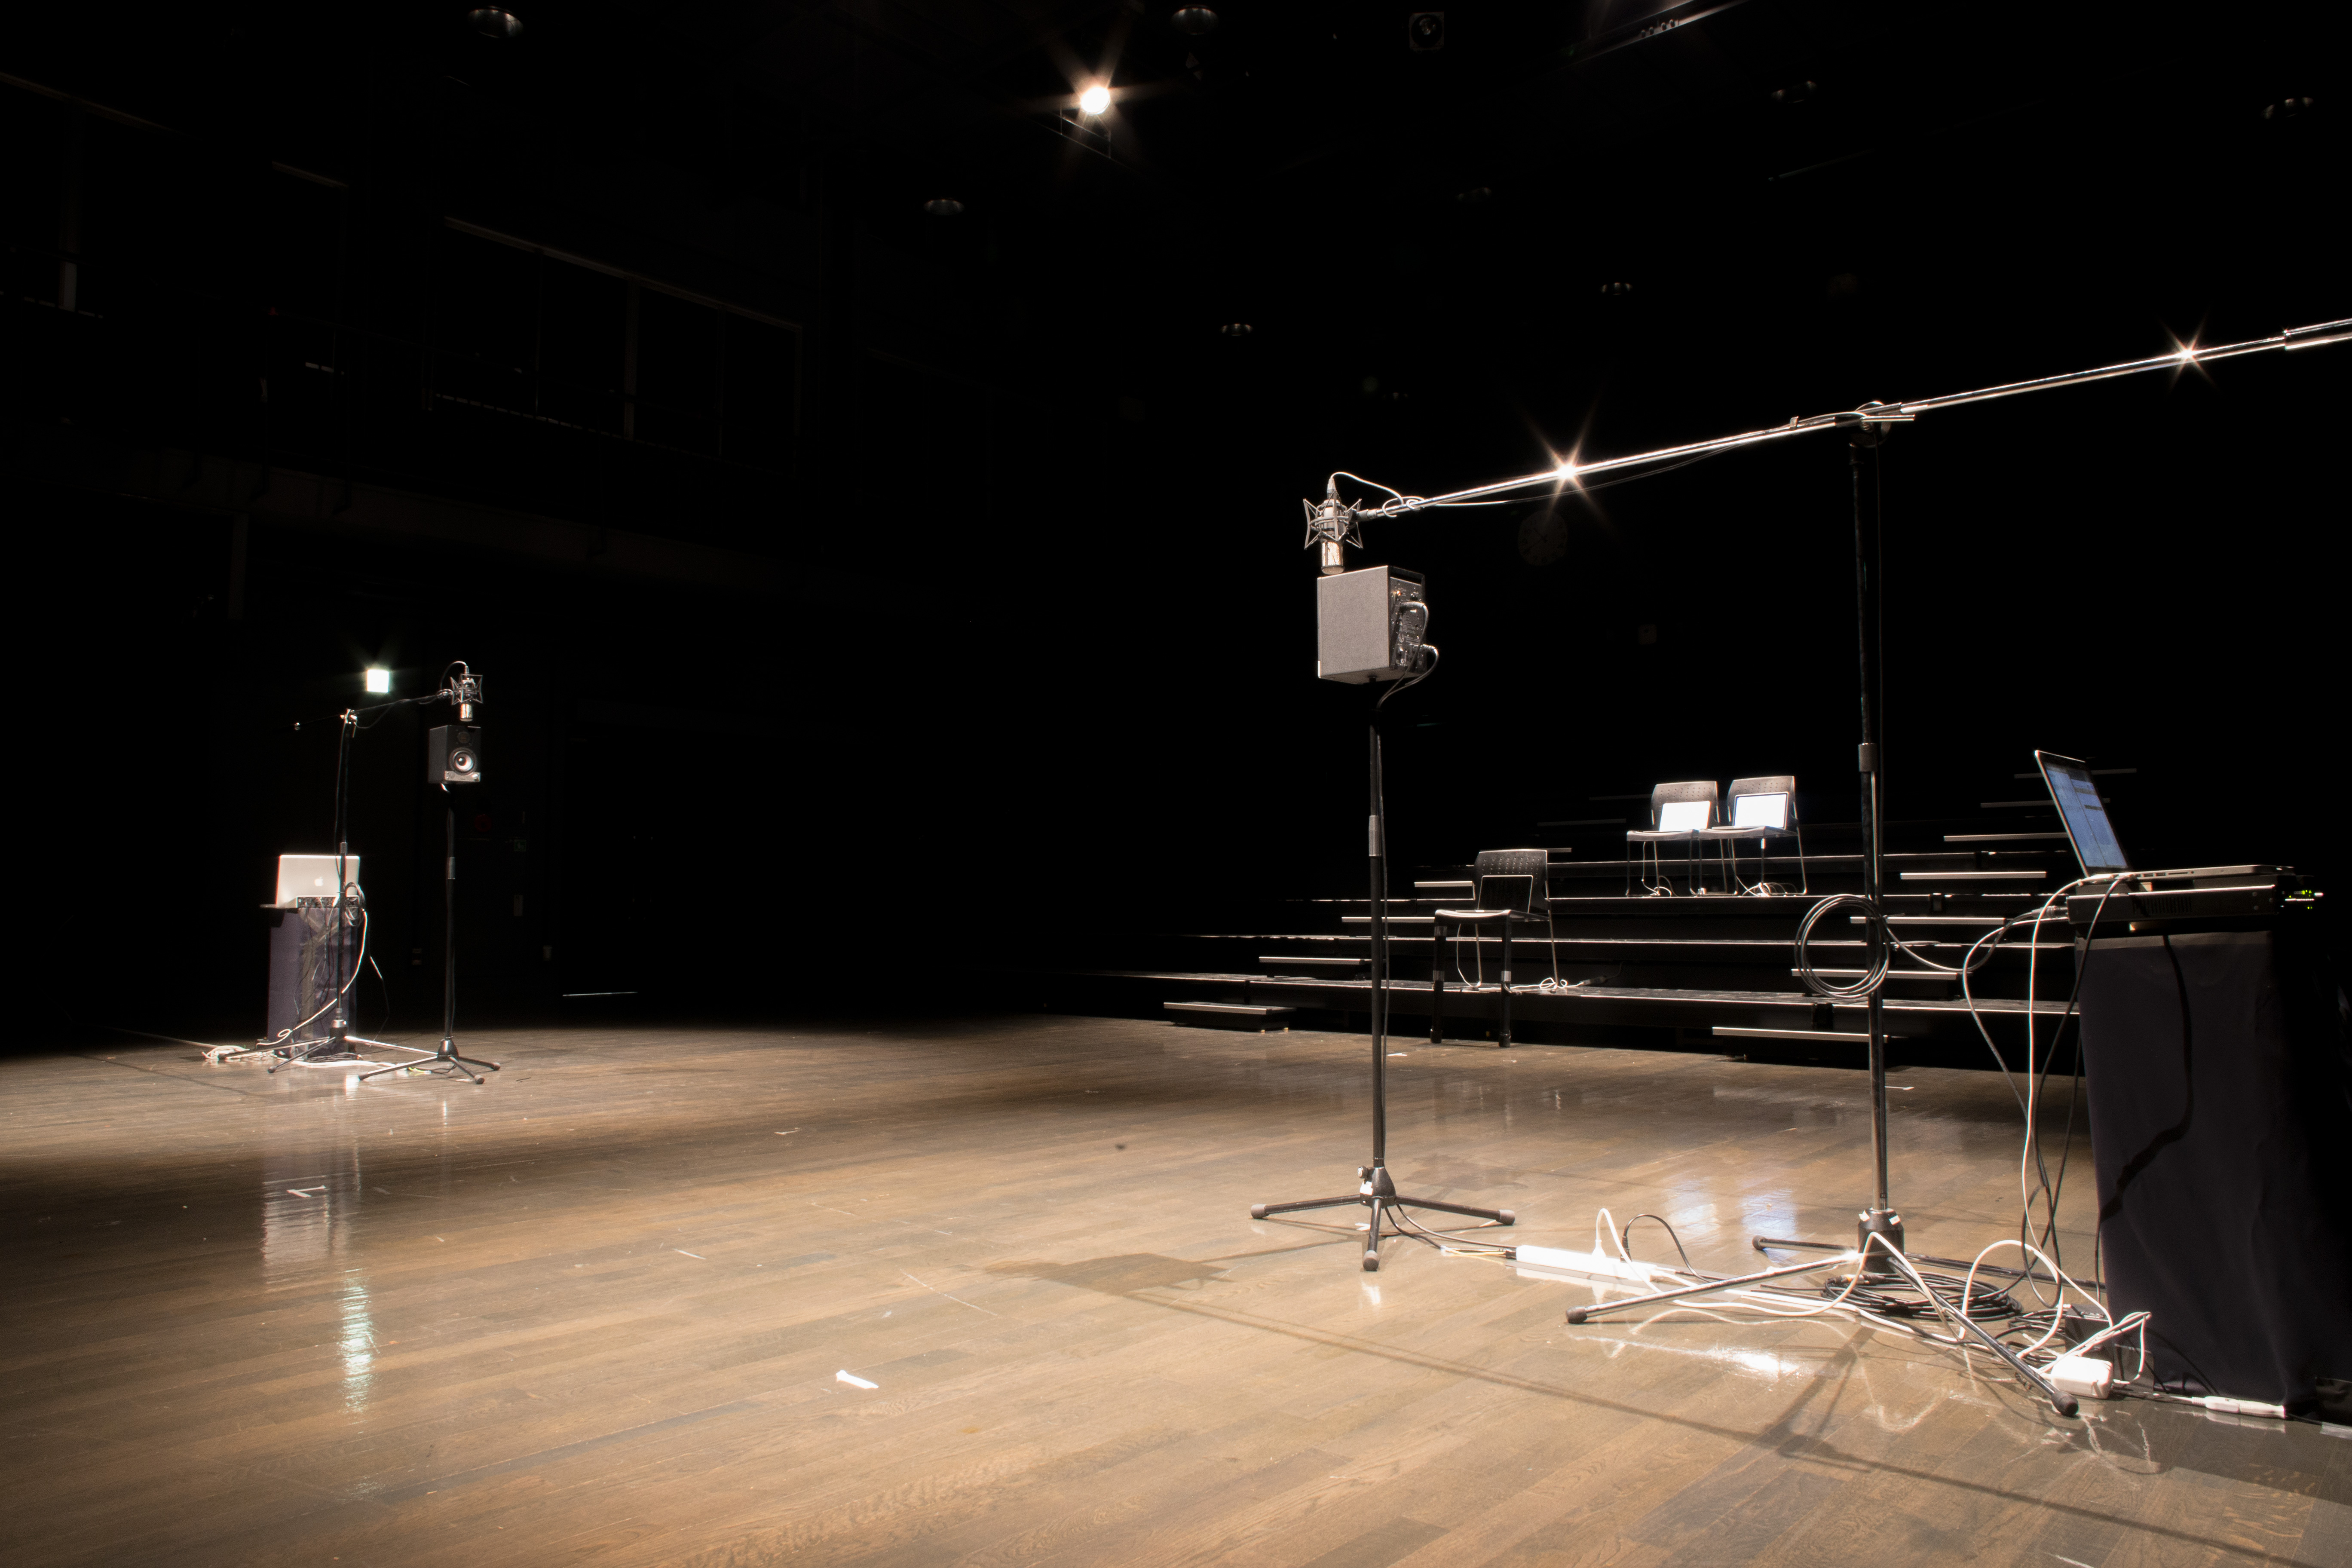
\includegraphics[width=1.00000\textwidth]{img/postpast1.jpg}~

\section{比較と考察}\label{ux6bd4ux8f03ux3068ux8003ux5bdf}

「Acoustic Delay (⇔)
Memory」と「送れ\textbar{}遅れ/post\textbar{}past」における大きな違いは「装置の分離」にあると考える。\\
比較の単純さのために後者のPC1,2の部分を取り出して考えると、それぞれの部分はスピーカー、マイク、オーディオインターフェース、PCが結線されており、PC1とPC2はハードウェア的に完全に分離されている。\\
つまり、個別の装置は受け取ったデータを送り返すだけの「通信装置」として機能する。\\
しかし2台の装置がそれぞれ同じデータを送り返し続けることで同じデータが保持され、結果的に「記憶装置」としての機能が成立する。\\
本来的に音響遅延線という装置も同じデータを受取り送信し続けることで記憶装置としての機能を持っていた。しかしそれは一台のハードウェアの中での通信であり、外見を見ればやはり1つの装置でしか無い。\\
しかし通信の繰り返しでデータの保存ができるという根本的な原理を考えると装置が2台以上に分離していても同じ機能を作ることが可能であり、その状態こそ通信と記憶の曖昧な状態を作り出すことが可能だと考え、2台に分けることにした。

\chapter{制作手順と技術的解説}\label{ux5236ux4f5cux624bux9806ux3068ux6280ux8853ux7684ux89e3ux8aac}

\section{実際の制作スケジュール}\label{ux5b9fux969bux306eux5236ux4f5cux30b9ux30b1ux30b8ux30e5ux30fcux30eb}

\begin{itemize}
\tightlist
\item
  6月:音響遅延線をテーマに作品制作を決定
\item
  7月:使える技術についての検討、無線通信技術や海中音響通信技術などの勉強
\item
  8月:適応フィルタ、低レイテンシーハードウェアの検証など
\item
  9月:千住キャンパス第7ホールで展示することを決定、音声入力と読み上げを使ったシステムも入れることを決める
\item
  10月:後半は第7ホールでの実地検証、読み上げシステムの実装
\item
  11月:展示
\end{itemize}

\section{制作に用いられた技術}\label{ux5236ux4f5cux306bux7528ux3044ux3089ux308cux305fux6280ux8853}

\subsection{音響遅延線メモリー部分}\label{ux97f3ux97ffux9045ux5ef6ux7ddaux30e1ux30e2ux30eaux30fcux90e8ux5206}

\subsubsection{信号処理のブロック・ダイヤグラム}\label{ux4fe1ux53f7ux51e6ux7406ux306eux30d6ux30edux30c3ux30afux30c0ux30a4ux30e4ux30b0ux30e9ux30e0}

イラレとかで書きます。。。

\subsubsection{位相偏移変調}\label{ux4f4dux76f8ux504fux79fbux5909ux8abf}

装置が2台に分かれるにあたって、従来の音響遅延線の仕組みをそのまま使おうとすると、マイクから受信した時に相手の信号と自分が発信した信号が混ざってしまうという問題点がある。今回はそれを2台の装置での使用周波数帯域を変更することで混線しないようにした。\\
周波数を変更するための変調方式には、載せる搬送波の振幅に信号を対応させる振幅偏移変調(ASK)、周波数変化に対応させる周波数偏移変調(FSK)、位相の変化に対応させる位相偏移変調(PSK)、振幅と位相を両方変化させる直行位相振幅変調(QAM)など様々な方式があるが、今回はQPSK、もしくは4QAMと呼ばれる、2bitのデータを位相の45°、135°、225°、315°の4状態に割り当てる方式を採用した。

(図)

図のように、基準となる位相から45°、135°、225°、315°がそれぞれデータの00、01、10、11に対応する。

\subsubsection{実際の実装方法}\label{ux5b9fux969bux306eux5b9fux88c5ux65b9ux6cd5}

主な実装には関数型音声処理言語のFAUST(Functional-AUdio-STream)を利用した。\\
FAUSTはフランスの音響研究機関、GRAMEの開発した言語であり、サンプル単位でのデジタル音声処理を非常に抽象的に記述することや、一度C++にコンパイルされてからスタンドアロンアプリケーション、Max/MSPやPuredataなど様々な環境上で動作させることができるという特徴を持つ。

今回はほとんどの音声処理部分をFAUSTで記述し、Cycling'74
Max上でリアルタイムにコンパイルできるfaustgen\textasciitilde{}という環境を使用した。Maxは主に波形の確認等デバッグのために用いられた。\\
FAUSTを選択した理由としては構想当初の段階でスマートフォン上のブラウザや音声入出力の遅延の少ない小型コンピュータ(Bela\footnote{Beaglebone
  Black})上で動作させることも想定しており、様々なプラットフォームで同じ音声処理を共通したコードで使いまわせるというメリットが大きかったためである。\\
結果的にはFAUSTはすべてMax上で動作させる形になったが、FAUSTで記述したコードは最適化された形でコンパイルされるため(正確なベンチマークなどの比較はしていないが)比較的低負荷で動作させることが可能であったなど、幾つかのメリットは合ったと考える。

\subsubsection{使える技術と使えない技術}\label{ux4f7fux3048ux308bux6280ux8853ux3068ux4f7fux3048ux306aux3044ux6280ux8853}

今回、実装するに

適応フィルタに於けるマルチパス除去などをしようとすると遅延が生じることなど

\subsection{読み上げによる仮想遅延線メモリー}\label{ux8aadux307fux4e0aux3052ux306bux3088ux308bux4eeeux60f3ux9045ux5ef6ux7ddaux30e1ux30e2ux30eaux30fc}

PuredataとAppleScriptでの読み上げ機能\\
スクリーンショットとか

\chapter{メディア考古学的メディアアート制作}\label{ux30e1ux30c7ux30a3ux30a2ux8003ux53e4ux5b66ux7684ux30e1ux30c7ux30a3ux30a2ux30a2ux30fcux30c8ux5236ux4f5c}

本章と次章においては卒業制作を作ったアーティストとしての立場というよりも、メディア考古学の研究をする立場、あるいはメディアアートについて研究する立場として俯瞰して自分の作品、あるいはそれを取り巻く環境について考察したい。\\
(なぜか書くべきか・・・)

\section{メディア考古学とは}\label{ux30e1ux30c7ux30a3ux30a2ux8003ux53e4ux5b66ux3068ux306f}

序論でも述べたように、メディア考古学とは特定の学問領域を指すのではなく学問のアプローチである。\\
序論で引用した太田の定義に加えて共通する特徴を挙げるのであれば、メディアの歴史を語る際にはよく、何が技術的に新しかったかを挙げ、またそのテクノロジーが与えた文化への影響を考察する、と言った態度が取られる。これは裏返せば新しい技術が登場することによって新しい文化が作られていく、いわゆる技術決定論的な立場を暗黙的に取っている事が多い。\\
これに対してメディア考古学的アプローチを取るものは新しいメディア装置が生まれる際に何か文化からの暗黙的な要請によって新しくテクノロジーが生み出されることも含め、より技術と文化の発展の相互作用を注意深く精査する。また同時代での注目だけではなく、歴史上で文化的に同じような言及がされていたりしないかを調べたりなど、時代を横断することで歴史観を見直すこともある。

中心的な研究者として挙げられるのはエルキ・フータモ、ユシ―・パリッカ、ジークフリード・ツィーリンスキー、自分で名乗ることはないもののフータモらが引用することも多いフリードリヒ・キットラーやその教え子であるウォルフガング・エルンストなどが挙げられる。\\
正確にはアプローチが異なるというよりも、ツィーリンスキーが自分の研究を「anarcheology」(アナーキー考古学)と呼んだように、自らの領域を厳格に定義しない事自体がメディア考古学の特徴となっている。

今回筆者の作品の考察をするにあたっては、そのように微妙に異なるアプローチの中から、代表的な研究者であるエルキ・フータモと、聴覚文化(音響再生産、複製技術)への数少ないメディア考古学的アプローチの研究として挙げられている、ジョナサン・スターン「聞こえくる過去」\autocite{stern:audiblepast}のアプローチを主に参考とした。

両者の研究態度にももちろん違いは存在するので、簡単にその概要を述べる。\\
フータモは(後述するが)元々文学領域で使われる用語であった「トポス」概念を拡張し、様々な年代のメディアで現れる共通した文化的言及を探し出す。\\
例えば「妖精エンジンを分解する」と題した項で「機械のブラックボックスの中で働く``小人''という表現」を中心として「見えざる神の手」「その時背後では?」のようなメディア装置の広告だったり、風刺画の中などに現れる定形表現を見つけ出し、歴史に共通する人間のメディアに対する態度を表出させてるとも言えるし、ある共通した項目を抜き出した新しいメディア史の記述ということもできる。

スターンの記述は、「聞こえくる過去」に於いては「音響再生産技術(Sound
Reproduction
Technology)」、一般的にはレコードやテープなどの複製技術と呼ばれるものについての言及にとにかく集中しているものの、それをイヤー・フォノトグラフと呼ばれる時代的に音響再生産技術の始まる直前の物を取り上げたり、聴診器や、電信のような再生産以前の技術と交えて議論したり、レコードのような複製物と死に対する観念に集中して議論したり、とにかく多面的な考察がなされる。\\
もうちょっと書きます。。。

\section{デジタル記憶装置はメディア考古学で掘れるのか}\label{ux30c7ux30b8ux30bfux30ebux8a18ux61b6ux88c5ux7f6eux306fux30e1ux30c7ux30a3ux30a2ux8003ux53e4ux5b66ux3067ux6398ux308cux308bux306eux304b}

\subsection{デジタル記憶装置に対する文化的言及}\label{ux30c7ux30b8ux30bfux30ebux8a18ux61b6ux88c5ux7f6eux306bux5bfeux3059ux308bux6587ux5316ux7684ux8a00ux53ca}

しかし、本作品の制作アプローチを二者のアプローチと比較しようとした時に大きな違いが出てくる。

そもそもは取り上げる装置の違いに起因する。音響遅延線だけではなく「デジタル記憶装置」という分類のものには「文化的な言及や現象」が存在していない事が多い。

その理由は主に2つである。

\begin{enumerate}
\def\labelenumi{\arabic{enumi}.}
\tightlist
\item
  記憶装置とは感性に対して直接作用するメディアでないこと。
\item
  デジタル記憶装置は扱う内容が極めて抽象化(エンコード)されること。
\end{enumerate}

「メディア考古学 ―過去と未来の対話のために―」の中で取り上げられる装置の実例を挙げると、万華鏡、ピンボールマシン、ゾートロープ(岩井俊雄の作品)、フォノグラフ(ポール・デマリニスの作品)などが挙げられる。\\
ピンボールマシンはともかく、それ以外の三者はすべて視覚や聴覚など、五感に対して何らかの作用を持つ装置であることは確かである。\\
しかし、デジタル記憶装置というものはデータをすべて一度0/1の並びに変換してその並びを保存する。\\
つまり保存するデータは言葉でも良いし、音楽でも画像でも、なんでもよい。\\
そのため、ハードディスクやフラッシュメモリ、そしてもちろん音響遅延線もレコードであったり写真のような文化を構成する一部としては考察し難い。

例えば最初は記録メディアがカセットテープであったウォークマンのことを考えてみると、1999年にフラッシュメモリ式のネットワークウォークマンと呼ばれるシリーズが発売され始める。\\
初期ウォークマンをカセットテープに付随する文化史の中に並べることはできるかもしれないが、フラッシュメモリにおいても同じ事が言えるのだろうか?\\
筆者自身はこれは不可能だと考える。その理由は先ほどから述べているように単にフラッシュメモリという記録メディアの保存できるものの種類が広範であることが大きい。\\
フラッシュメモリ型ウォークマンの与えた文化的影響についての考察はできるかもしれないが、フラッシュメモリ単体でそれが与えた文化的影響を考察するのは散漫にならざるをえない。\\
このように、デジタルメディアはその汎用性が故に記録、再生装置、もしくは記録/再生する内容とセットにしなければ考察する対象にならないのである。

それに加えて、音響遅延線メモリーが動作していたのは初期のコンピュータなので、フラッシュメモリのように広く一般に普及したわけでもなく、各マシンによって詳細な構造もそれぞれ異なるという点もある。

\subsection{音響遅延線メモリー開発者自身による言及}\label{ux97f3ux97ffux9045ux5ef6ux7ddaux30e1ux30e2ux30eaux30fcux958bux767aux8005ux81eaux8eabux306bux3088ux308bux8a00ux53ca}

ここで一度製作者(アーティスト)としての立場で振り返る。

エッカートのインタビューの時点ではエッカートが自分の耳で聞き、それを繰り返し唱え続けることで長期記憶になるという話が挙げられていた。(音響遅延線について唯一文化的言及ということができるかもしれないもの)\\
しかし装置の実装、実践をしている内にこれは実は違うと思うようになった。\\
なぜなら短期記憶の繰り返しによって長期記憶ができるというのはブラウン管のような焼付きに近い(もう直接自分の引用するか)

結果的にこの言及が作品の制作上のシステムに影響することはなかったと考える。\\
それよりはGoogleドキュメントの音声入力のシステムであったりとか、現代の状況のほうが強く影響を与えていたような気がする。

〜つづく〜\\
結局、「送れ|遅れ/post|past」において、筆者は「手段は問わないデジタル装置」は逆説的に「何らかの伝達と認識の手段の存在」によってその機能が保証されていて、「その装置の機能の持つ手段から文化的な意味を''勝手''に読み出してより見える形にする」ということをしている、そしてその文化的意味が表出するためには「装置が現在の文化においては役に立たない」ことが必要となる

ということを丁寧に書きたい

\section{メディア考古学的アプローチでのメディアアート
-城一裕らの「車輪の再発明プロジェクト」から}\label{ux30e1ux30c7ux30a3ux30a2ux8003ux53e4ux5b66ux7684ux30a2ux30d7ux30edux30fcux30c1ux3067ux306eux30e1ux30c7ux30a3ux30a2ux30a2ux30fcux30c8--ux57ceux4e00ux88d5ux3089ux306eux8ecaux8f2aux306eux518dux767aux660eux30d7ux30edux30b8ux30a7ux30afux30c8ux304bux3089}

フータモらの挙げるようなメディアアーティスト(ポール・デマリニスや岩井俊雄ら)は自らのアプローチをメディア考古学と言うわけではなく\footnote{ただしポールデマリニスは1997年のNTTICCでの展示は「-Archaeology
  of Media-」というタイトルを付けている。}、フータモら研究者が考察する際に挙げているだけである。\\
それに比べて数少なく、作品(作品でなくとも、何かしらの「制作」プロジェクト)において明示的に「メディア考古学」の名前を上げているプロジェクトとして、2015年にNTTのICCで行われたメディアアートを取り上げる通年展示「オープン・スペース2015」での日本の岐阜県にあるメディアアートを専門にした大学院である情報科学芸術大学院大学(通称IAMAS)でのプロジェクト「車輪の再発明プロジェクト」がある。THE
SINE WAVE
ORCHESTRAのメンバーかつ研究者でもある城一裕を中心に、クワクボリョウタ、瀬川晃、松井茂ら講師と学生によって行われたプロジェクトである。

\begin{quote}
このプロジェクトでは実践を通じて歴史を読み替え,ありえたかもしれない「今」をつくりだします.淘汰されてしまった過去のメディアを再考察することで新しい現在のメディアへの理解を深める「メディア考古学」を足がかりに,視聴覚メディアを中心とした様々なメディアの形づくられてきた過程を調べ,その機能や役割が歴史的に固定される前の可能性について理解を深めます.\\
そして,コンピュータやネットワークを取り入れた個を主体としたものづくりの潮流である「パーソナル・ファブリケーション」以降の技術・社会環境において,この理解を芸術表現に活用する方法を,多様な作品制作の下地となる技法として提案します.\\
例えば,聴覚メディアの古典的な存在ともいえるレコード,その機能や役割を,画面上で描いた波形を溝として盤面に直接刻み込むという〈技法〉を用いて制作したいくつかの〈作品〉,を通じて再考するように,マス・メディアにおいては顕在化しなかったメディアの可能性を「再発明」します.\\
\autocite{iamas:RIWP}
\end{quote}

本作品の制作に於いては少なくとも制作当初の段階(7月頃)において「メディア考古学的アプローチ」という点に自覚的に制作を行っていた点、「あり得たかもしれない今を作り出す」という点に引っ張られていた気はする。\\
しかし作ったものはおそらくあり得たかもしれない今というものですら無いかもしれない?

車輪の再発明プロジェクトにおいて挙げられる特徴はデジタルファブリケーション、パーソナル・ファブリケーションなどモノづくりに使われる技術を導入することで新しいあり得たかもしれない歴史が作れるという読み替えである。

そこから受けた影響としては、そもそも水銀使えないし、現代の状況で音響遅延線作ったら否が応でも異なる物が出来上がる、その時存在しなかった無線技術の導入をするっていうところはそこの影響をかなり受けていると思われる。

研究者としての立場に戻ると、でもある意味これって技術決定論の方に寄るのでは?

\chapter{メディア考古学的メディアアート史考察}\label{ux30e1ux30c7ux30a3ux30a2ux8003ux53e4ux5b66ux7684ux30e1ux30c7ux30a3ux30a2ux30a2ux30fcux30c8ux53f2ux8003ux5bdf}

\section{メディアアートと呼ばれるモノとの交わり}\label{ux30e1ux30c7ux30a3ux30a2ux30a2ux30fcux30c8ux3068ux547cux3070ux308cux308bux30e2ux30ceux3068ux306eux4ea4ux308fux308a}

ここからはメディアアートと呼ばれるものとメディア考古学、そして本作品の関係についての考察を行いたい。\\
「メディアアートと呼ばれるもの」と書き続けているのは、「メディアアート」という言葉の定義が非常に曖昧であるからである。\\
現状メディアアートと言っても元来の意味であった「ニューメディアアート」の文脈を引き継ぐ、いわゆる新しい技術(例えば2016年に於いてはバーチャル・リアリティやディープラーニングなどはそれらに当てはまるだろう)をアート作品に用いるものや、日本の代表的なメディアアートの美術館であるNTTインターコミュニケーションセンターでの年間展示「オープン・スペース」の2016年のタイトルが「メディア・コンシャス」であるように表現に関わるテクノロジーや素材(メディウム)が現代においてどういう文化的意味を持ちうるかについて言及する傾向のものなど、幾つかの分類が可能なようにも見える。

しかしながら本論考では敢えてメディアアートの作品群を分類し、その中のどこに本作品が位置するか、のような言及の仕方は避けたいと考える。\\
なぜならそれら複数のジャンルに跨るものも当然存在するし、そのような線引きを行うことで見えなくなってしまう要素も存在すると考えるからである。(あいまいなので変えたい)

日本のメディアアート観に対する統一見解も未だまとまったものが存在するところではないが、馬定延「日本メディアアート史」などで幾つかまとめようとする試みは出てきている。\\
しかし「日本メディアアート史」でのアプローチは、一般的な美術史の様に代表的な作品を列挙するのではなく、背景的に起こった出来事(例えば大阪万博など)、セゾンや草月アートセンター、NTTのICCなど舞台となった場を中心として、メディアアートとは何なのかを探るようなアプローチとなっている。\\
このようなアプローチを取った理由について馬は序章においては

\begin{quote}
1970年代以降の日本のエレクトロニックアート紹介において、美術館における展覧会でなく、博覧会の名前が羅列されているのはなぜだろうか。なぜこれらの場を並べずには、日本のメディアアートの軌跡を語る事ができなかったのだろうか。
\end{quote}

\begin{quote}
こうした問題意識から、本書は個別の作家や作品ではなく、その背景をなす時代像に焦点を当ててみる。すなわち、本書はメディアアートの作品論と作家論を可能な限り排除して書かれたメディアアート史である。このような方法論が、究極的には、すべての表層的な要素、移り変わっていく背景を取り除いたあとに残る、メディアアートの本質たるものを強調することを目的にしていることは言うまでもない。
\end{quote}

と述べているし、またあとがきにおいては本書中で挙げられた作品写真は本文で言及されていないものばかりかつ、作品の説明などはなく最低限の情報しか載せていないことに触れた上でこう述べる。

\begin{quote}
筆者の明確な意図は、これらの画像を通して、何がメディアアートなのかではなく、むしろその定義不可能性を提示し、読者に問いかけることである。
\end{quote}

と、ある種明確にメディアアートの定義は不可能だと言い切っている。\\
実は本書は日本を代表するメディアアーティストである藤幡正樹についての研究から始まり、彼を中心として起きた出来事の歴史をまとめた論文が元になっていると本人も語っている\footnote{2015/12/12\textasciitilde{}13の千住
  Art Path
  2015(東京芸術大学千住キャンパス制作・研究発表展)での毛利嘉孝とのトークにおいて。またあとがきの最後でも遠回しであるが日本で研究する目的が藤幡について研究したかったから、ということを述べている。}。その為この本もかなり引いた目線で語っているとは言え日本のメディアアートの全てを包括して語っているとは言い難い。

しかしながら私はこの「引いた目線」、歴史を一つの観点で見定めようとせずに、起きた事象を冷静に見つめ、通底する物を引き出そうとする姿勢はメディア考古学的アプローチと強く結びつくところがあると考える。その為本作品のメディアアートの中での位置づけを考える際の大きな参考の一つとしたい。

何が「引いた目線」がメディア考古学的視点と結びつくとか、と言うのは特にフータモのメディア考古学観、特に彼の言う拡張された「トポス」概念である。

トポス概念とはもともと文学の中の常套句のようなものであり、メディア考古学を考察するにあたってフータモはこの概念を拡張している。\\
例えばバーチャル・リアリティにおける「没入感」などの言葉や「複雑な仕組みの機械の様子を表現するのに妖精や小人がマシンを動かしている比喩」などがある。

要するに、歴史は現代の状況から記録を見返して作られるものであり、現代の状況が歴史観の形成に与える影響は大きい。例えばメディア史であれば技術の与えた影響が文化を変えて、また文化の要請が新たな技術を生み出すことで変化し続けることと同様に、メディアアートは時代を取り巻く技術及び文化の状況が変化することでその都度歴史観が大きくひっくり返される可能性があるのではないだろうか。

\section{メディアアート史に作品を位置づけることは可能か}\label{ux30e1ux30c7ux30a3ux30a2ux30a2ux30fcux30c8ux53f2ux306bux4f5cux54c1ux3092ux4f4dux7f6eux3065ux3051ux308bux3053ux3068ux306fux53efux80fdux304b}

さて、それでは仮にメディアアート史というものが存在したとして、その文脈の中に本作品を位置づけることが可能かどうかということを考えてみたい。

\chapter{まとめ}\label{ux307eux3068ux3081}

ここまで、卒業制作「送れ|遅れ/post|past」について、メディア考古学的アプローチでの作品制作に対する考察と、メディア考古学的アプローチからメディアアート史に対して作品を位置づけることについての考察を行ってきた。

制作においては本作品はフータモやスターンの挙げてきたようなメディア考古学的アプローチとも、

\section{結び}\label{ux7d50ux3073}
